\documentclass[a4paper, 12pt]{report}

%%%%%%%%%%%%
% Packages %
%%%%%%%%%%%%

\usepackage[english]{babel}
\usepackage{packages/sleek}
\usepackage{packages/sleek-title}
\usepackage{packages/sleek-theorems}
\usepackage{packages/sleek-listings}
\usepackage{dirtree}
\usepackage{graphicx}
\usepackage{caption}
\usepackage{subcaption}

%%%%%%%%%%%%%%
% Title-page %
%%%%%%%%%%%%%%

\logo{./resources/pdf/logo.pdf}
\institute{Universidad Politécnica de Cartagena}
\faculty{Ingeniería Telemática}
%\department{Department of Anything but Psychology}
\title{Aplicaciones en Internet}
\subtitle{Web de recomendación de películas}
\author{\textit{Autores}\\\textsc{Álvaro Herández Riquelme}\\ y \textsc{André Yermak Naumenko}}
%\supervisor{Linus \textsc{Torvalds}}
%\context{A long time ago in a galaxy far, far away...}
\date{\today}

%%%%%%%%%%%%%%%%
% Bibliography %
%%%%%%%%%%%%%%%%

\addbibresource{./resources/bib/references.bib}

%%%%%%%%%%
% Macros %
%%%%%%%%%%

\def\tbs{\textbackslash}

%%%%%%%%%%%%
% Document %
%%%%%%%%%%%%

\begin{document}
    \maketitle
    \romantableofcontents



    \newpage
    \newpage

    \chapter{Introducción}
    Este documento tiene como objetivo explicar el funcionamiento de la aplicación web de recomendación de películas llamada \texttt{El Recomendador}.

    El proyecto incluye funcionalidades clave como la autenticación de usuarios, gestión de perfiles, un catálogo dinámico de películas, un sistema de puntuación y comentarios, y algoritmos avanzados para la recomendación y el ranking de películas. Además, se ha diseñado una interfaz intuitiva y una arquitectura robusta basada en PHP, JavaScript, MATLAB y SQL.

    Cada capítulo abordará las distintas funcionalidades y aspectos técnicos del proyecto de forma sintética y clara para poder así comprender el funcionamiento al completo de la aplicación.
    \chapter{Index}

    En primera instancia, el usuario accederá a esta página. En ella, el usuario se puede encontrar una portada con una breve descripción de la web, y en ella va incluida dos formularios, una de registro y otra de inicio de sesión. Se ha optado por una portada simple y minimalista para que el usuario pueda acceder rápidamente a la web.
    \section{index.html}

    A nivel técnico, la página principal se compone de un formulario de inicio de sesión y un formulario de registro. Ambos formularios están diseñados como una extensión HTML del archivo \textit{index.html} de tal modo que son gestionadas por separado y se pueden encontrar en los directorios \textit{/auth/register.php y /auth/registerform.html} para el registro y \textit{/auth/login.php y /auth/loginform.html} para el inicio de sesión.

    Para el fondo hemos elegido una animación discreta de una luz recorriendo la pantalla, esto se puede asemejar a los salvapantallas de los televisores con el logo DVD que cuando chocan con un borde, cambia su camino.

    \begin{figure}[h!]
        \centering
        \begin{subfigure}{0.45\textwidth}
            
\includegraphics[width=\textwidth]{resources/img/index.png}
            \caption{Inicio de la web.}
            \label{fig:index}
        \end{subfigure}
        \hfill
        \begin{subfigure}{0.45\textwidth}
            
\includegraphics[width=\textwidth]{resources/img/salvapantallasdvd.png}
            \caption{Inspiración del salvapantallas DVD.}
            \label{fig:savescreen}
        \end{subfigure}
        \caption{Comparación entre el index de la web y el salvapantallas DVD.}
        \label{fig:comparacion}
    \end{figure}

    \textit{¿Por qué se ha optado por hacer eso?}

    La razón principal es la posibilidad de implementar un formulario HTML pero que no esté visible al cargar la página, sino que se muestre al hacer clic en el botón correspondiente. La respuesta al botón se realiza mediante \textit{JavaScript}, pero la implementación de dos formulario, con mismo estilo que aparezca como respuesta a un \textit{script}, nos ha llevado a la llamada externa de dichos formularios y que se gestionen por separado en distintos documentos y además a la creación de un archivo de estilos llamado \textit{core.css}, que será un archivo con los estilos comunes a todas las páginas de la web.
    \section{core.css}
    En este archivo podemos encontrar la configuración común a todas las páginas de la web. En él se han definido los estilos de los formularios, las cabeceras, los pie de página, la fuente y el tamaño de la letra...

    Todas las páginas de la web heredarán dichos archivos, y si en alguna página se quiere modificar algún estilo, se puede hacer de forma individual en el archivo de la página correspondiente.

    \begin{figure}[h!]
        \centering
        \begin{subfigure}{0.45\textwidth}
            
\includegraphics[width=\textwidth]{resources/img/header.png}
            \caption{Inicio de la web.}
            \label{fig:header}
        \end{subfigure}
        \hfill
        \begin{subfigure}{0.45\textwidth}
            
\includegraphics[width=\textwidth]{resources/img/footer.png}
            \caption{Inspiración del salvapantallas DVD.}
            \label{fig:footer}
        \end{subfigure}
        \caption{Comparación entre el index de la web y el salvapantallas DVD.}
        \label{fig:elementoscompartidos}
    \end{figure}

    Un ejemplo claro es la reutilización de recursos como el header y el footer. En la figura~\ref{fig:elementoscompartidos} se puede ver la cabecera y el pie de página de la web. Ambos elementos se han ido utilizando en todas las páginas de la web.
    \chapter{Sección de la autenticación}
    \section{check\_session.php}
    \section{loginform.html y registerform.html}
    \section{login.php}
    \section{logout.php}
    \section{register.php}

    \chapter{La carpeta Pages: las páginas visibles}
    \section{catalog.php}
    \begin{figure}[H]
        \centering
        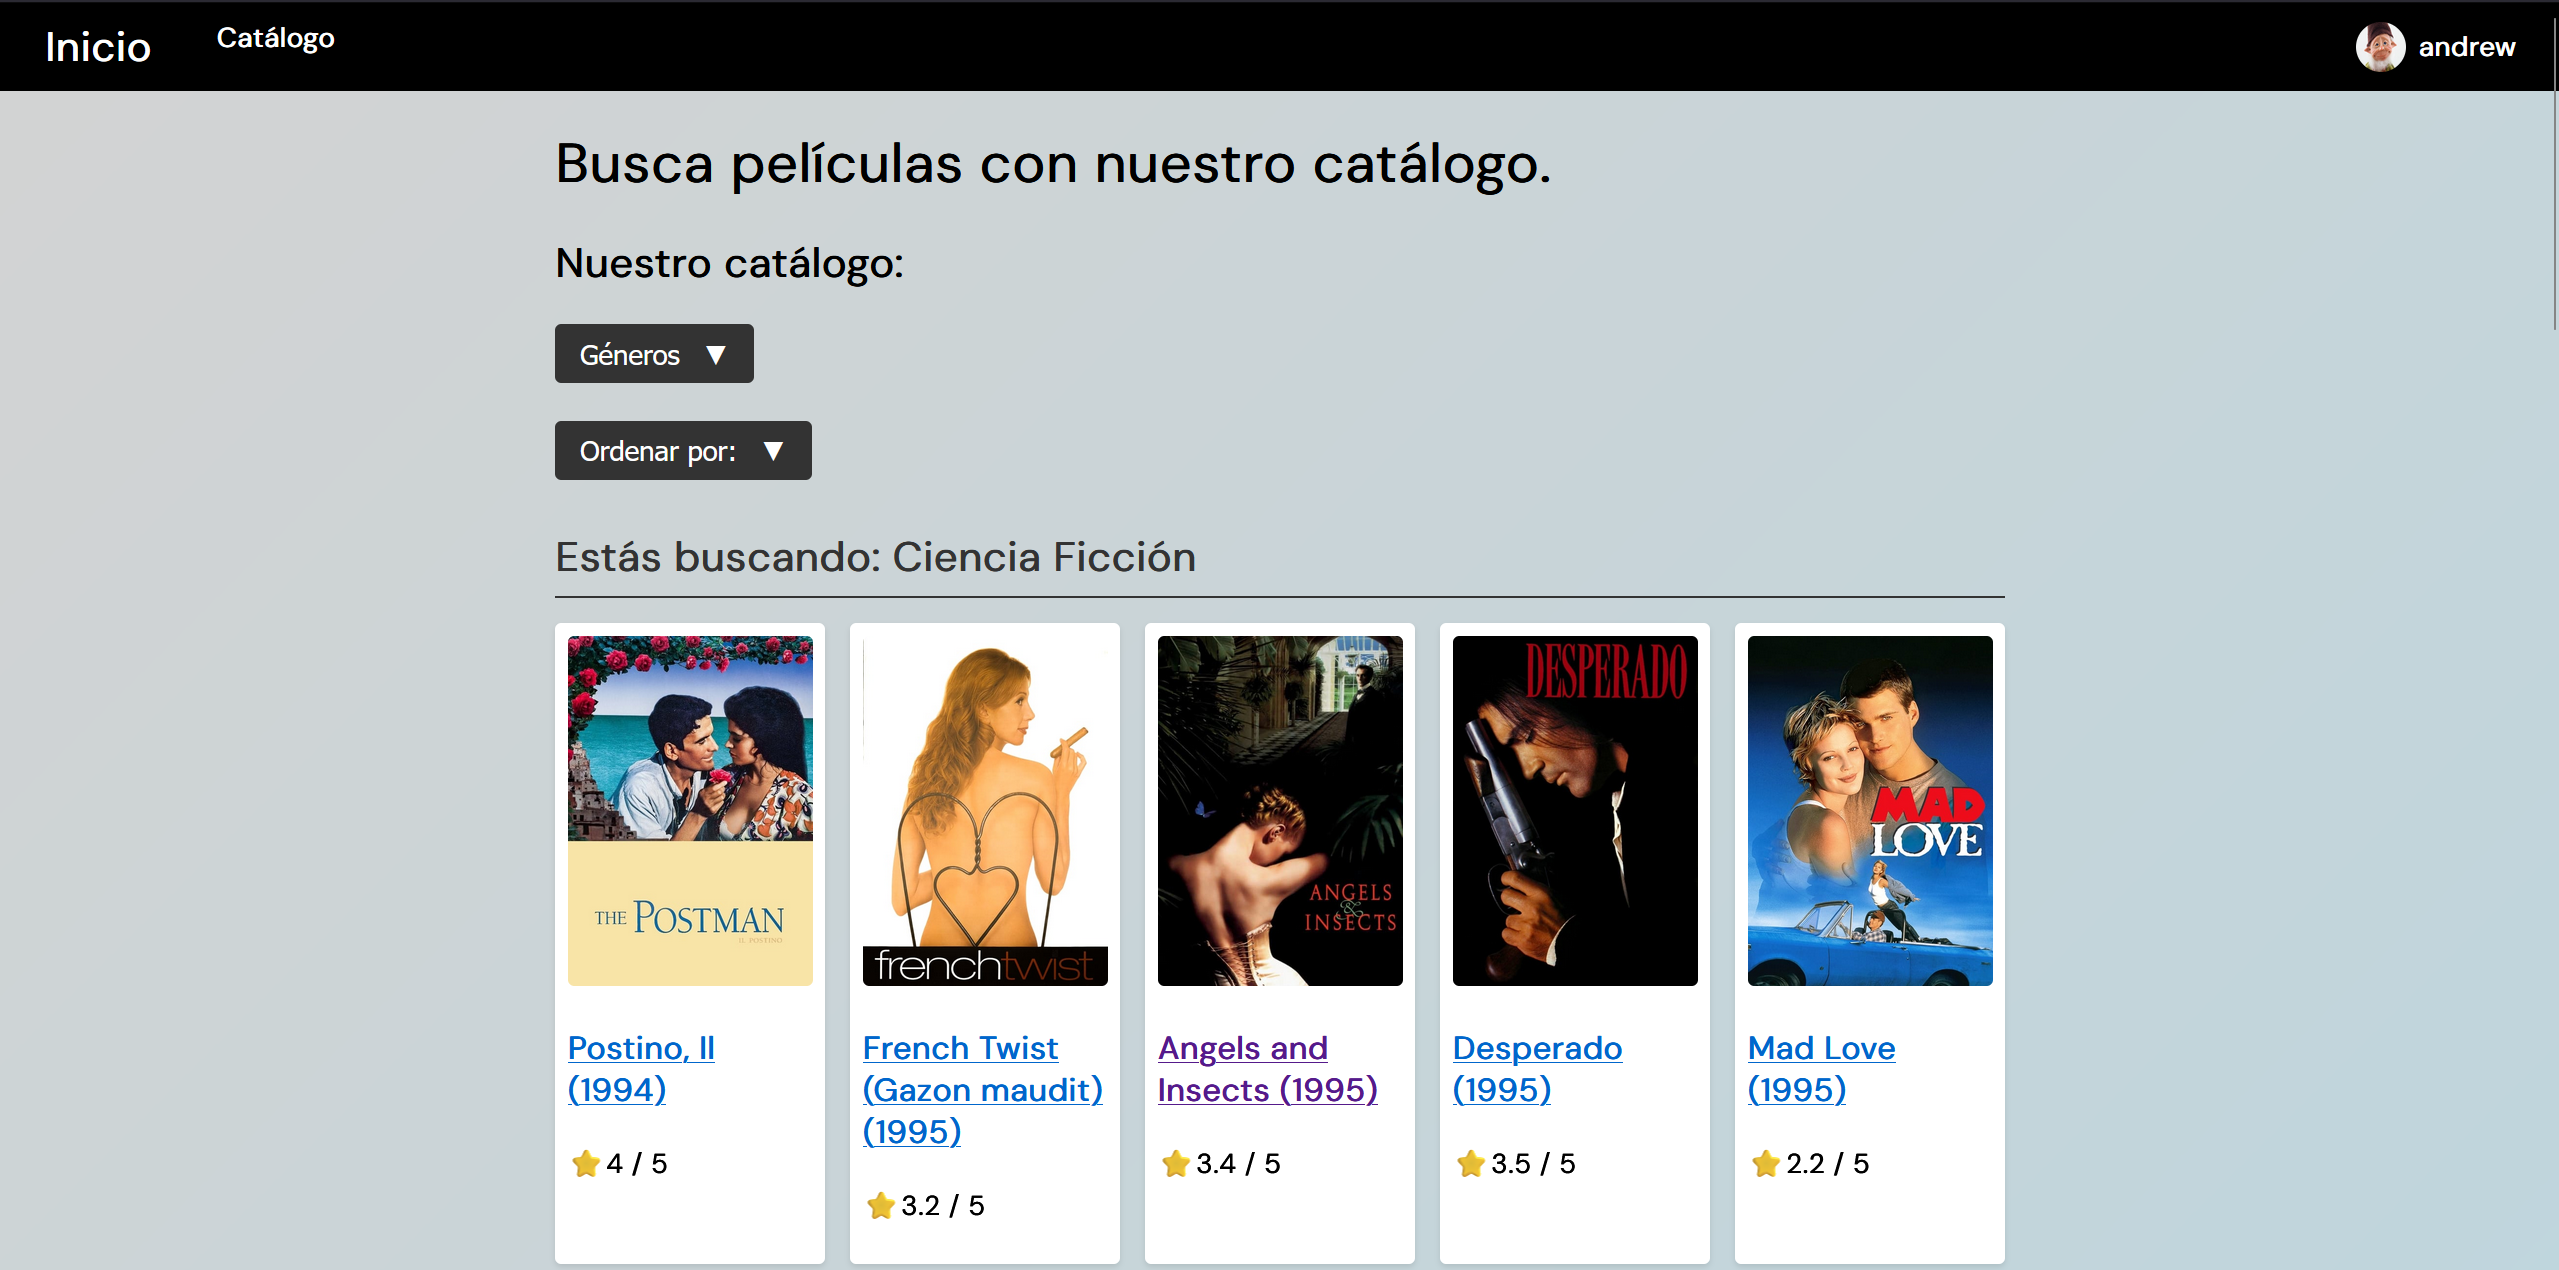
\includegraphics[scale=0.20]{resources/img/catalog.png}
        \caption{Página catalog.php.}
        \label{fig:catalog}
    \end{figure}
    \section{edit\_profile.php}
    \begin{figure}[H]
        \centering
        \includegraphics[scale=0.20]{resources/img/edit\_profile.png}
        \caption{Página edit\_profile.php.}
        \label{fig:edit}
    \end{figure}
    \section{main.php}
    \begin{figure}[H]
        \centering
        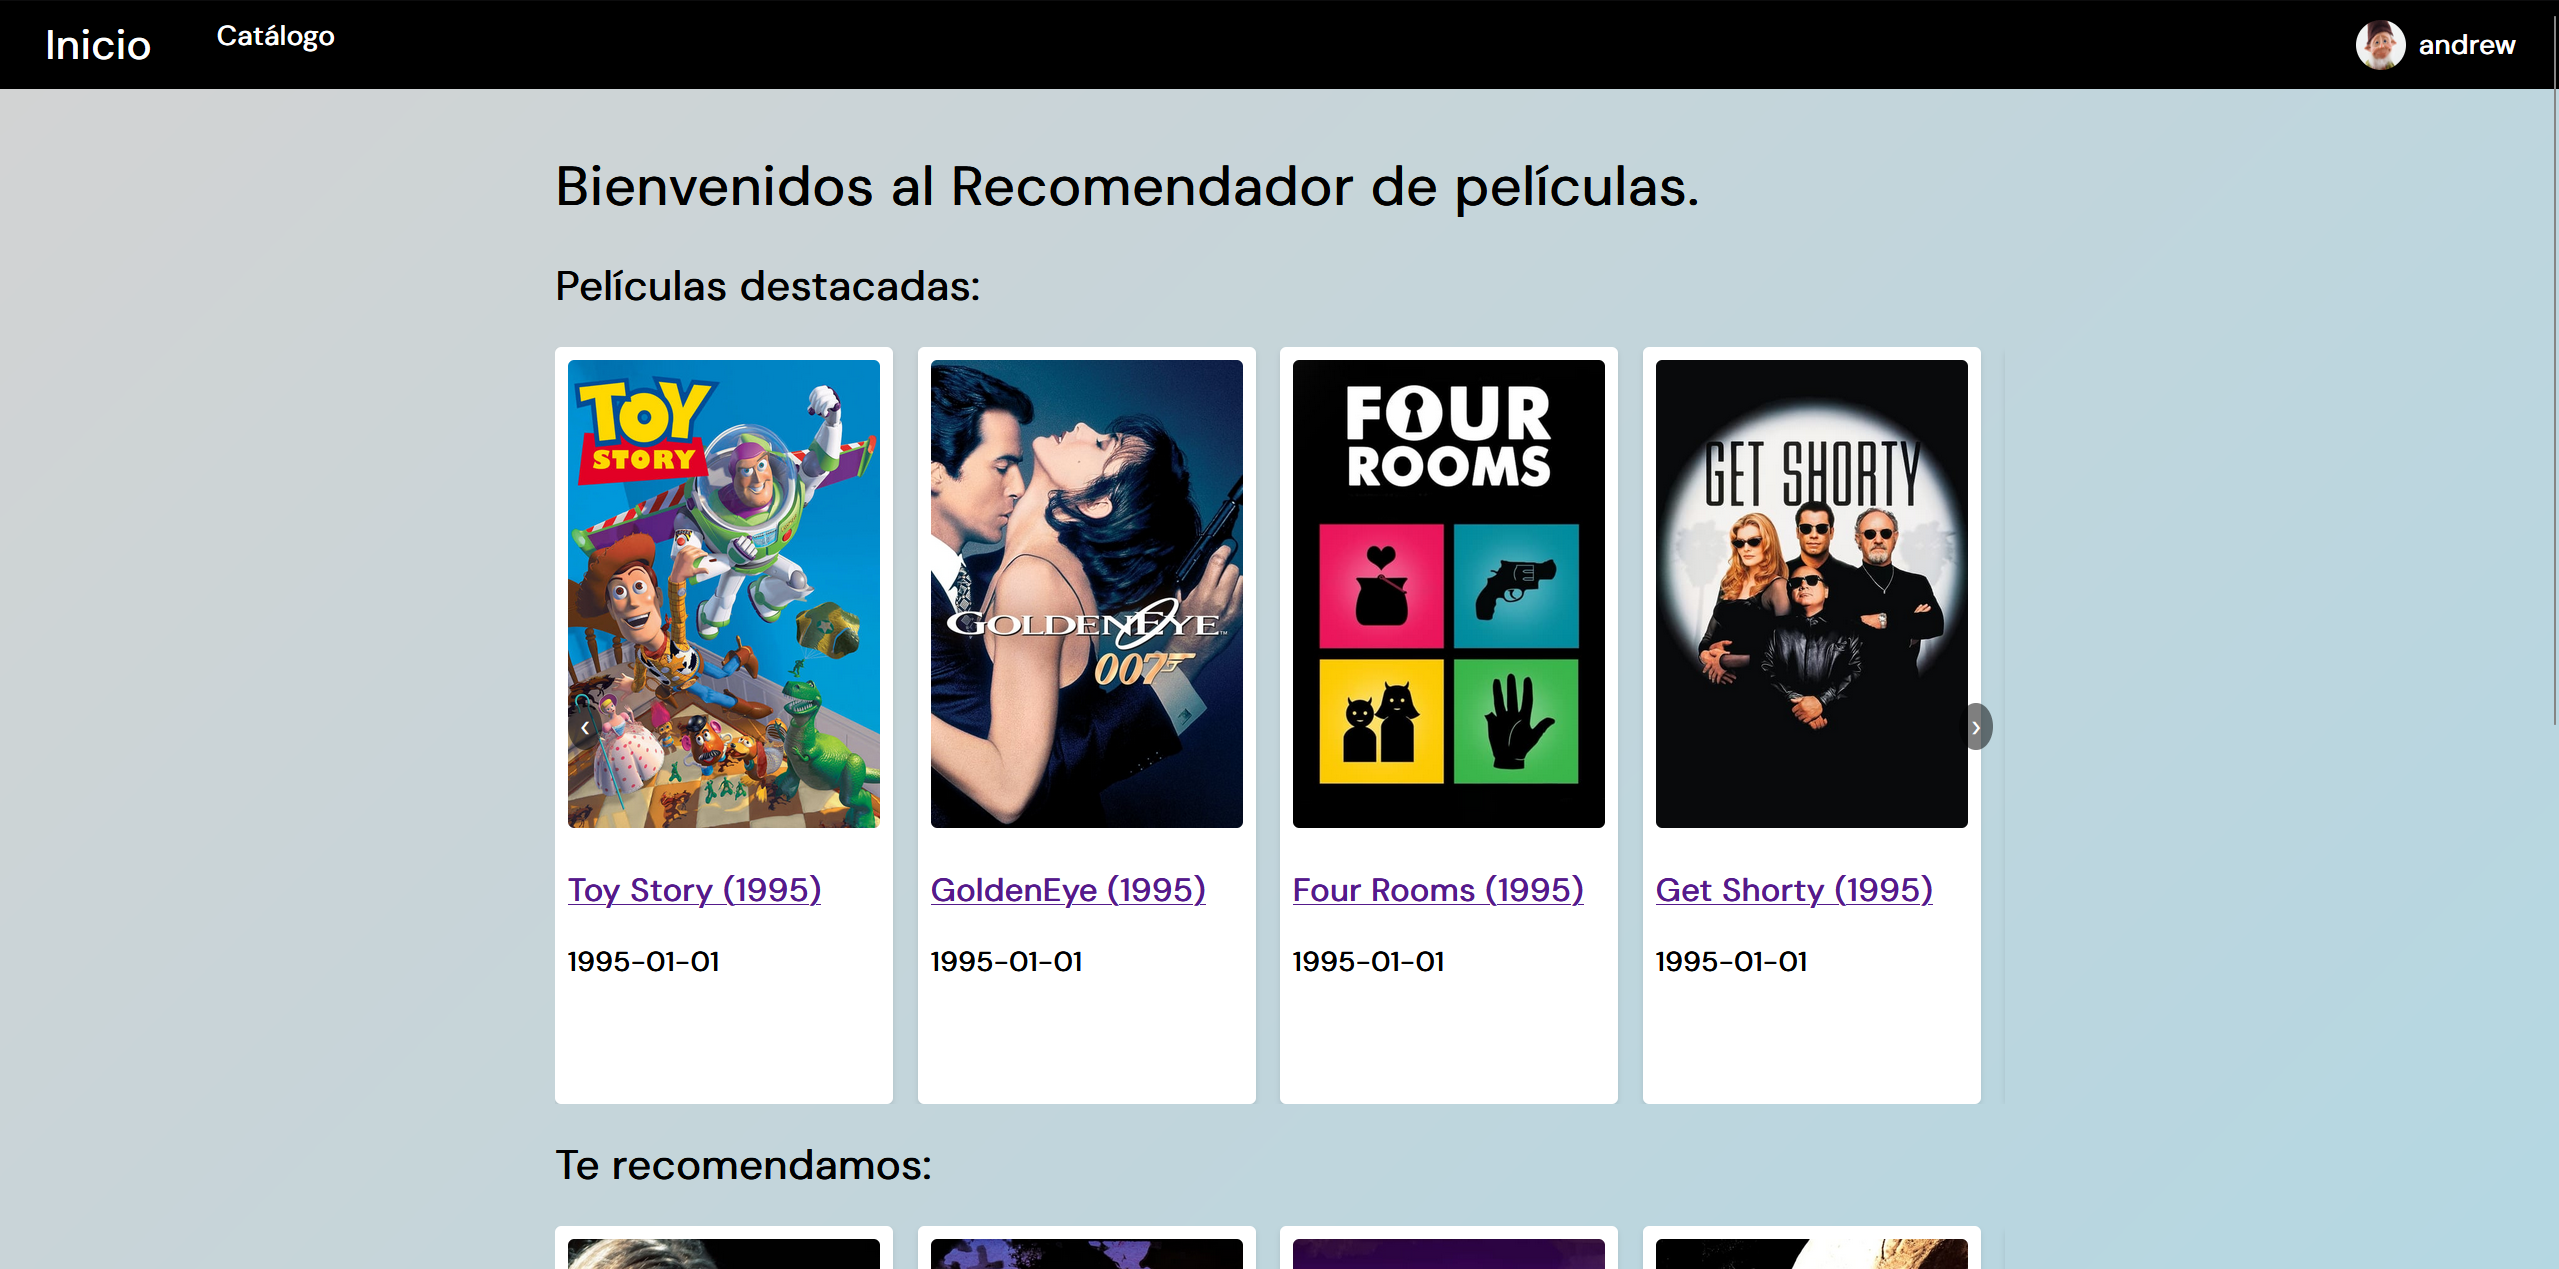
\includegraphics[scale=0.20]{resources/img/main.png}
        \caption{Página main.php.}
        \label{fig:main}
    \end{figure}
    \section{pelicula.php}
    \begin{figure}[H]
        \centering
        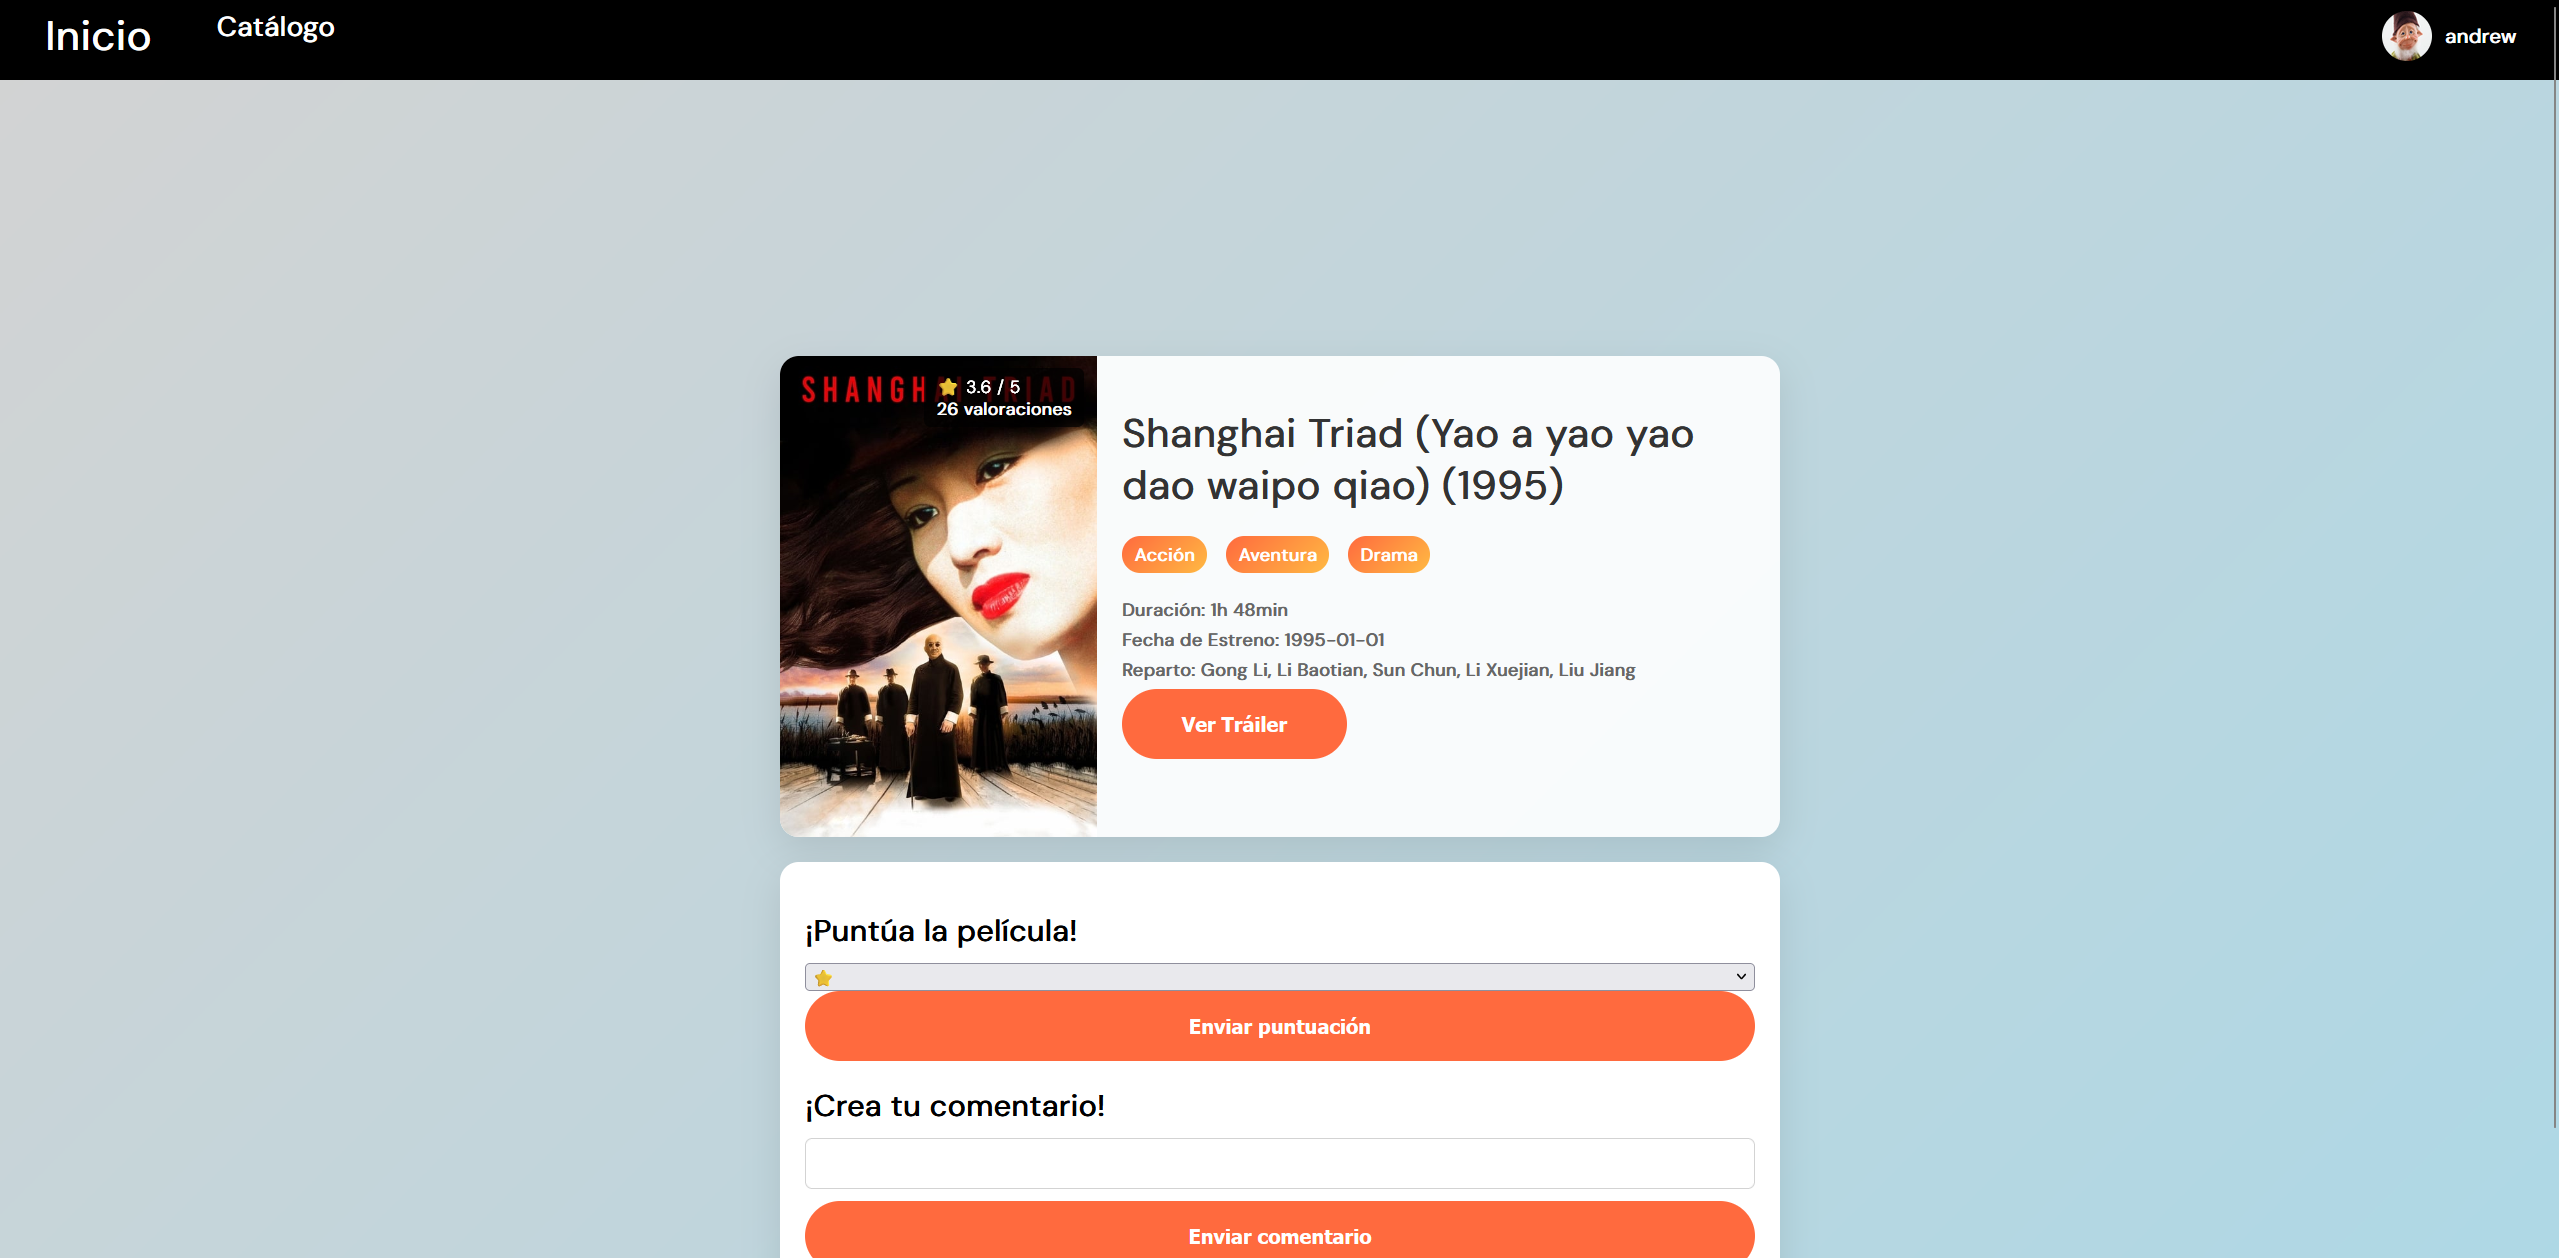
\includegraphics[scale=0.20]{resources/img/movie.png}
        \caption{Página pelicula.php.}
        \label{fig:pelicula}
    \end{figure}
    \section{profile.php}
    \begin{figure}[H]
        \centering
        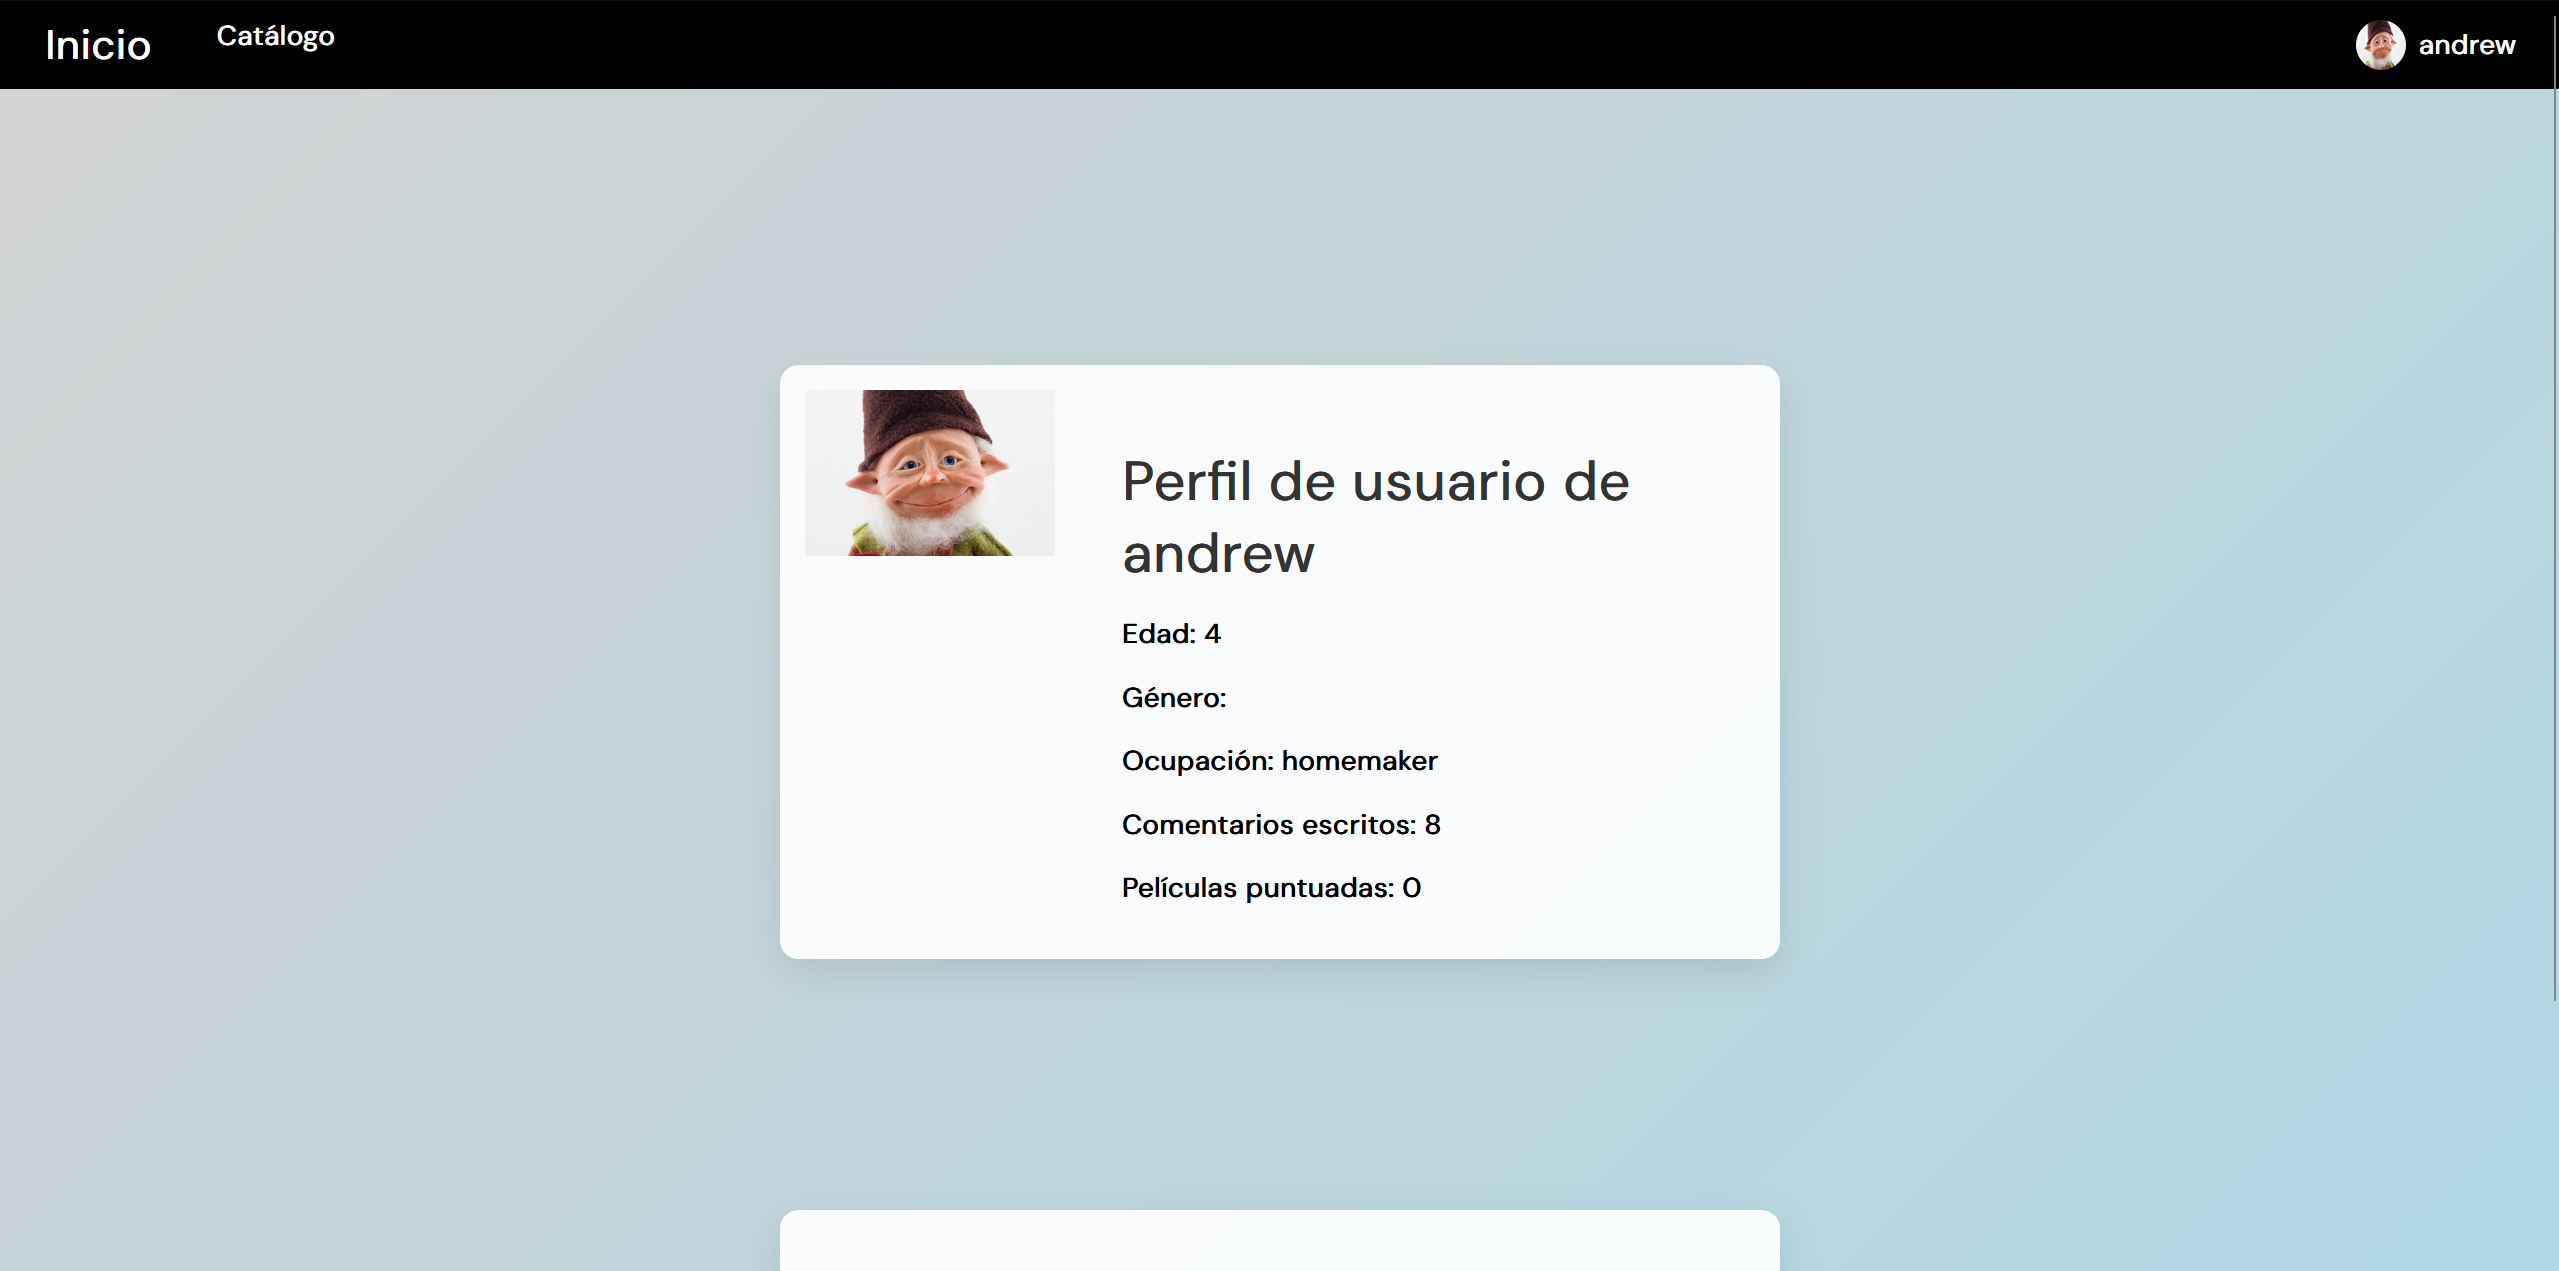
\includegraphics[scale=0.20]{resources/img/profile.png}
        \caption{Página profile.php.}
        \label{fig:profile}
    \end{figure}

    \chapter{Uso de las peticiones GET y POST PHP}
    \section{cargar\_comentarios.php}
    \section{change\_profile.php}
    \section{check\_password.php}
    \section{crear\_comentario.php}
    \section{puntuar\_pelicula.php}


    \chapter{Includes}
    Se ha decidido crear un directorio \textit{includes} la cual contenga scripts PHP que se van a utilizar en varias páginas de la web. De esta forma, se evita la repetición de código y se facilita la gestión de los mismos.
    \section{common.php}
    Este script se encarga principalmente de recolectar toda la información para las películas, desde llamadas a API hasta consulta de base de datos de las puntuaciones de cada película.
    \section{conectar.php}
    Se centraliza la conexión a la base de datos en este script. De esta forma, se evita la repetición de código y haciendolo más legible.
    \section{genres.php}
    Consulta a la base de datos de información de los géneros para una película \textit{i}.
    \section{movies.php}
    Realiza una consulta paginada a una base de datos para obtener una lista de películas, opcionalmente filtradas por género, y devuelve los resultados en formato JSON.

    \chapter{JavaScript}

    Los scripts de \textit{JavaScript} tiene una implementación variada, nos podemos encontar desde scripts sencillos para el index.html~\ref{fig:comparacion} hasta scripts combinados para poder cargar de forma asíncrona las imágenes de las peliculas.
 
    \section{carousel.js}
    Aunque nos hubiese gustado crear una implementación completa (scroll vertical "aparentemente infinto" y el carousel \cite{carousel}),
    \section{dropdownLogout.js}
    DropdownLogout es un scprit sencillo que se encarga de escuchar el click en el nombre de usuario para desplegar 2 botones, "Cerrar sesión" y "Mi perfil".
    \section{lazyload.js}
    Para la carga de imágenes, nos hemos enfrentado a un problema crucial y es que la página no se quede colgada durante largos segundos hasta que la carga de todas las imágenes se complete, para ello hemos decidido implementar \textit{Lazy Loading}\cite{lazyloading}. Con ello solucionamos todos los problemas de carga de imágenes y la página funciona desde el instante 0 sin necesidad de que carguen todas las imágenes.
    \section{main.js}
    Este script sólo se encarga de la parte estética del \textit{index.html}, haciendo que la "luz" rebote contra los bordes de la ventana.

    \chapter{Matlab y los algoritmos}
    Los algoritmos en Matlab se han implementado desde la carpeta \textit{matlab}. En ella se encuentran los archivos \textit{getData.m} y \textit{updateRecommendation.m} entre otros, que son los encargados de la conexión con la base de datos y de la actualización de las recomendaciones, respectivamente.
    Cabe recalcar que no se ha podido comprobar el funcionamiento de los algoritmos y su correcta implementación en la web, ya que no se ha podido correr un servidor de Matlab en la máquina local no tampoco del servidor ofrecido para la entrega.
    \section{Conexión BBDD con Matlab}
    La conexión a la base de datos se gestiona medinante 2 archivos, \textit{getData.m} ofrecido por el profesor, y \textit{updateRecommendation.m} . Todos esos datos son los que nos permiten procesar la información y realizar las recomendaciones.
    \section{main.m}
    En este archivo se centraliza toda la lógica de los algoritmos de recomendación y la puntuación Bayesiana. Recoge los datos necesarios y realiza las iteraciones necesarias para obtener los resultados. Posteriormente esos datos son enviados a la base de datos.
    \section{Algoritmo de puntaje con Bayesian Ranking}
    Para realizar el puntuaje con Bayesian Ranking, se ha utilizado la siguiente fórmula:
    \begin{equation}
        p_i = \frac{NR+n_ir_i}{N+n_i}
    \end{equation}    siendo $N$ el número total de películas, $R$ la puntuación media de todas las películas, $n_i$ el número de puntuaciones de la película $i$, $r_i$ la puntuación media de la película $i$, $m$ la puntuación media de todas las películas y $v$ la varianza de las puntuaciones de todas las películas.
    \newpage


    %%%%%%%%%%%%%%%%%%%%%%%%%%%%%%%%%%%%%%%%%%%%%%%%%%%%%%%%%%%%%%%%%%%%%%%%%%%%%%%%%%%%%%%%%%%%
    % ------------------TODO LO QUE ESTÁ ABAJO HAY QUE ELIMINARLO LUEGO----------------------- %
    %%%%%%%%%%%%%%%%%%%%%%%%%%%%%%%%%%%%%%%%%%%%%%%%%%%%%%%%%%%%%%%%%%%%%%%%%%%%%%%%%%%%%%%%%%%%
    \printbibliography

\end{document}
